\documentclass[../main/Feedback.tex]{subfiles}
\begin{document}
\section{Experiment Design}
%We used fNIRS because it is non-invasive with low sensitivity to motion artefacts, and with high temporal resolution, thus suitable for user trials. We combine the fNIRS, as an objective measure of mental workload with the subjective NASA-TLX as they are validated and reliable methods \cite{maior2015examining,hart2006nasa}. In addition, we decided to measure the emotional valence with the SAM questionnaire. This way we gather comprehensive information about how participants perceive the interfaces and relate it to the psychophysiological data. Furthermore, fNIRS is novel method for conducting usability studies, and as such we aim to assess its practicality.
%This study was looking at this.... The study used repeated measures within subjects design. 
%The depended variable was the objective workload, and the independent variable was the layout of the three web forms. 
We chose to focus our study of form filling on a car insurance claim scenario, as it was a) an example of an important web form that people encounter in everyday lives, b) involves careful thought rather than just entering data, and c) was in line the real concerns of an industry partner that wants to make their service as easy to use as possible. Video clips were used as the stimulus for filling in insurance claims during the study,  with a time gap, such that participants had to recall aspects of the accidents. These video clips provided all the necessary data for filling in the forms.
Further, the video clips were of the low-speed accidents and were carefully chosen to be lightweight avoiding any scenes of gore, injured bodies, or fatalities. We compared three alternative designs, described below, and measured performance, time to complete, emotional responses, and mental workload.

\subsection{Layout variations of web forms}
A total of 3 HTML/CSS variations of a standard web form for an insurance claim were produced, as shown in Figure \ref{fig:layout-variations}.
They were created to resemble an actual online insurance claim form, but excluded aspects such as brand and colour, to avoid these having an impact on the results.
All conditions included three main parts: 1) Personal information, 2) Accident information and 3) a summary of the accident.
The personal information, such as name, date of birth, etc, was given to participants on paper, such that they did not have to input personal information, nor would they have to apply additional mental workload to generate fake information.
%Because of ethical considerations, participants were presented with artificial personal details.
The accident information (part 2) consisted information about the time and location, and a series of drop down lists about the number of passengers and cars involved in the accident and the location of the damage on their vehicle.
The final part consisted of a text-area, where participants had to write an overall description of the accident, what led to it, and so on. 

Our control condition, index1, was simply a form that contained all three parts on one page. 
%The first investigated layout, referred as index1, consisted of the three division areas laid out with the summary of accident at the end.
The first experimental condition, index2, tested the hypothesis that beginning with a general summary of the accident (part 3 at the top) would reduce the level of mental workload overall for the form; summarising it would make subsequent box filling easier.
The second experimental condition, index3, tested the general design recommendation that breaking down a form into subforms (one for each part) would make it easier to fill out in stages. %had the same order as index1, with each division part situated on separate page (personal information on page 1, accident information on page 2 and summary on page 3).
Users navigated between the three parts of index3 using a submit button with the label``Next''.

%\subsection{Participants}


\subsection{Objective Measures}
Aside from recording time to complete each task, Hemodynamic data was recorded during each condition using the fNIRS300 device along with the COBI studio recording software developed by Biopac Systems inc.
The device consists of a headband with 4 infrared LED emitters and 10 infrared detectors.
The combination between them was used to calculate 16 channels which can measure the associated oxygenated (HbO), deoxygenated (Hbr) and total (Hbt) haemoglobin concentration in the PFC.
They operated on 730nm and 850nm wavelengths.
The emitter-detector separation was 2.5cm and the sampling rate was 2Hz.
The data from 3 participants was excluded due to recording problems.

\textbf{Data Processing} was performed using fnirSoft \cite{ayazfunctional}. 
A low-pass filter with cut off frequencies of 0.1 Hz, was used in order to remove physiological noise.
The NIRS signal was then processed with modified Beer-Lambert law\cite{cope1988system}, in order to calculate HbO, Hbr and Hbt.  
The correlation based signal improvement(CBSI) \cite{cui2010functional} method was applied to remove motion artefacts.
%\subsubsection{Feature Extraction/selection}
After data preprocessing, the mean and standard deviation for Hbo, Hbr and Hbt data was calculated from all channels.
%\begin{figure}[h]
%	\centering                                                                                                                                                                                             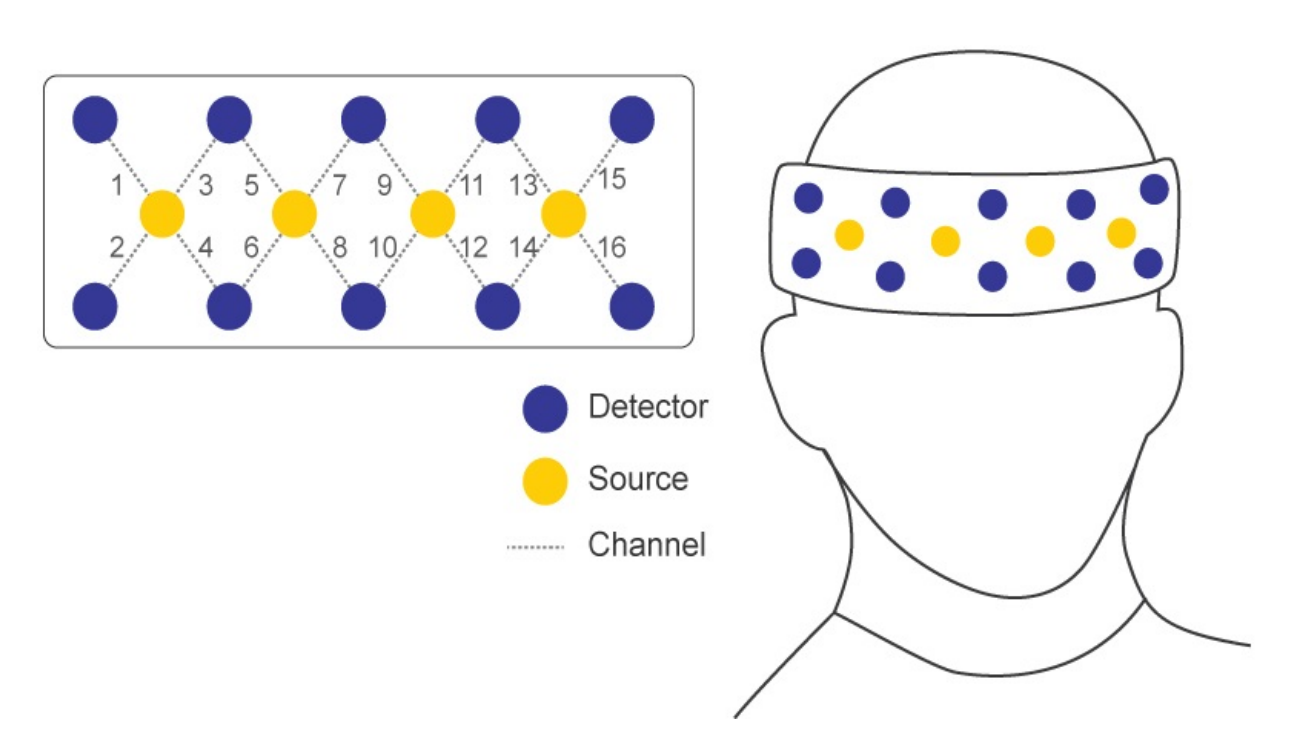
\includegraphics[width=0.7\linewidth]{../figures/source-detector-diagram}
%	\caption[fNIRS source-detector diagram]{The spatial arrangement of the source-detector pars placed on participants forehead.}
%	\label{fig:source-detector-diagram}
%\end{figure}


\subsection{Self-Reporting Measures}
To assess operator perceived workload we used the paper version of the multidimensional subjective workload scale NASA-TLX \cite{nasatlx}.
The individual scales are presented in the following order: Mental demand, Physical demand, Temporal demand, Performance, Effort, and Frustration.
The NASA-TLX scores were obtained from participants after completing each web form conditions. To capture participants emotional valence and arousal we used a 5 point self assessment mankin (SAM)\cite{bradley1994measuring} after each video and form-filling condition.  
%The participants were asked to fill the questionnaire after each video watched. 
%First they state their emotional valence(negative or positive) by choosing between 1 and 5, where 5 is strongly perceived positive emotion, and 1 is considered strong negative emotion. Then, they fill the arousal level scale, where 1 indicates low perceived arousal or boredom, and 5 signifies high perceived arousal or high level of excitement. Each of the subscales is supported by image visualisations illustrating the affective state.

%\subsubsection{Sound recording}
%The participants voice was recorded during the experiment using researchers mobile phone. The data was used to transcribe the user comments.

\subsection{Procedure}
A total of 15 right handed participants (5 female) with mean age of 26 (SD = 4.71) were recruited from the University of Nottingham.
%All of the participant were healthy, 
All participants were undergraduate or graduate students, had normal or corrected vision, and report no history of brain damage. %, however one suffered froom Von Willebraud disease, which impairs blood's ability to clot, and so their data was excluded from the study.
%Fourteen of them reported they have advanced computer literacy, five of them stated average computer literacy and one did not answer this question.
%All of the participants were current or graduated students. The ethics committee of the University of Nottingham approved this study.
To begin with, informed consent was obtained from the participants, and then, when ready, the fNIRS headband was placed and calibrated using a period of rest. Participants then followed the procedure illustrated by Figure \ref{fig:study-procedure}. 


\begin{figure}[h]
	\centering
	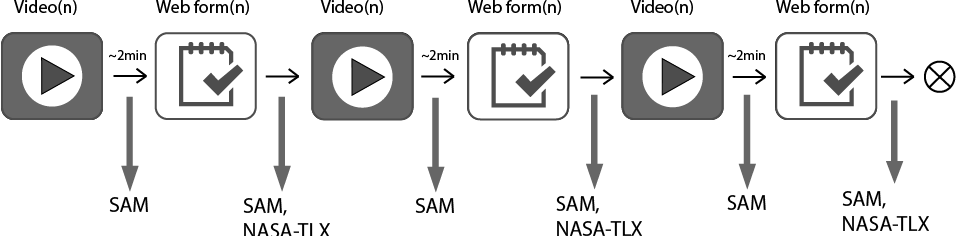
\includegraphics[width=\linewidth]{../figures/study-procedure}
	\caption[study procedure]{The image illustrates, the study procedure followed in this experiment.}
	\label{fig:study-procedure}
\end{figure}


The three study conditions were counterbalanced using Latin square, to avoid learning effects. Within each condition, participants first viewed a video clip, and then filled in a SAM test. SAM answers were informally monitored, as well as casual conversation between conditions, to check that participants werent experiencing distress from watching the videos. After a 2-minute gap, to allow for the accident to begin to decay from working memory, participants proceeded to fill in the current form condition (also counterbalanced). To conclude the condition, participants filled in a NASA-TLX form and another SAM test. 
%Also, because of ethical considerations that the participant should not enter personal data in the web form, a artificial personal credentials were provided, that she should fill in the web forms. 
%Fourth, after the video capture and the fNIRS device were started, participants were asked to relax, in order to record a baseline of the hemodynamic activity while participants are at rest. Next, they are asked to open one of the three videos, depending on the counterbalancing order. 
%They were instructed by the researcher to manually start certain condition or video. 
%After watching of the video was finished, participants fill SAM subjective scale. 
%Fifth, there was approximately 2 minute waiting period between the video and the web form filling task, so that participant's memory is not fresh. Finally, after participant completed the web form the NASA-TLX scales was given to be completed. 
This process was repeated three times, to complete the three conditions.% following the within subjects experimental design with counter balancing between the videos and the web forms.
The study then concluded with an informal debriefing interview.

\end{document} 